Nous avons dans un premier temps essayés de rendre notre implémention parallèle. Pour cela, il est nécessaire de s'intéresser aux problèmes posés par les tableaux de travail de $A$ et $B$, alloués une fois dans la fonction goto\_dgemm et passés aux sous fonctions.\\

Nous décidons de paralléliser le long de la dimension $M$, en ajoutant une directive "\#pragma omp parallel for schedule(static) shared(A\_packed, B\_packed, C\_aux, C)" dans goto\_dgepp afin de distribuer les appels à goto\_dgbp. Le tableau de travail de $B$ est déjà prêt et sera partagé entre les threads. Pour ceux de $A$ et $C$, nous allouons un tableau par thread, et utilisons un ordonnancement statique pour s'assurer de l'ordre d'accès des threads.\\
Le problème étant fixe en terme de quantité de calculs il se prête d'ors et déjà à un ordonnancement statique. Ensuite chaque thread se charge d'écrire dans son tableau pour s'occuper d'une partie de $C$. Notons que chaque thread s'occupe d'une partie de $C$ ce qui nous permet d'éviter toute synchronisation.

\begin{figure}
    \centering
    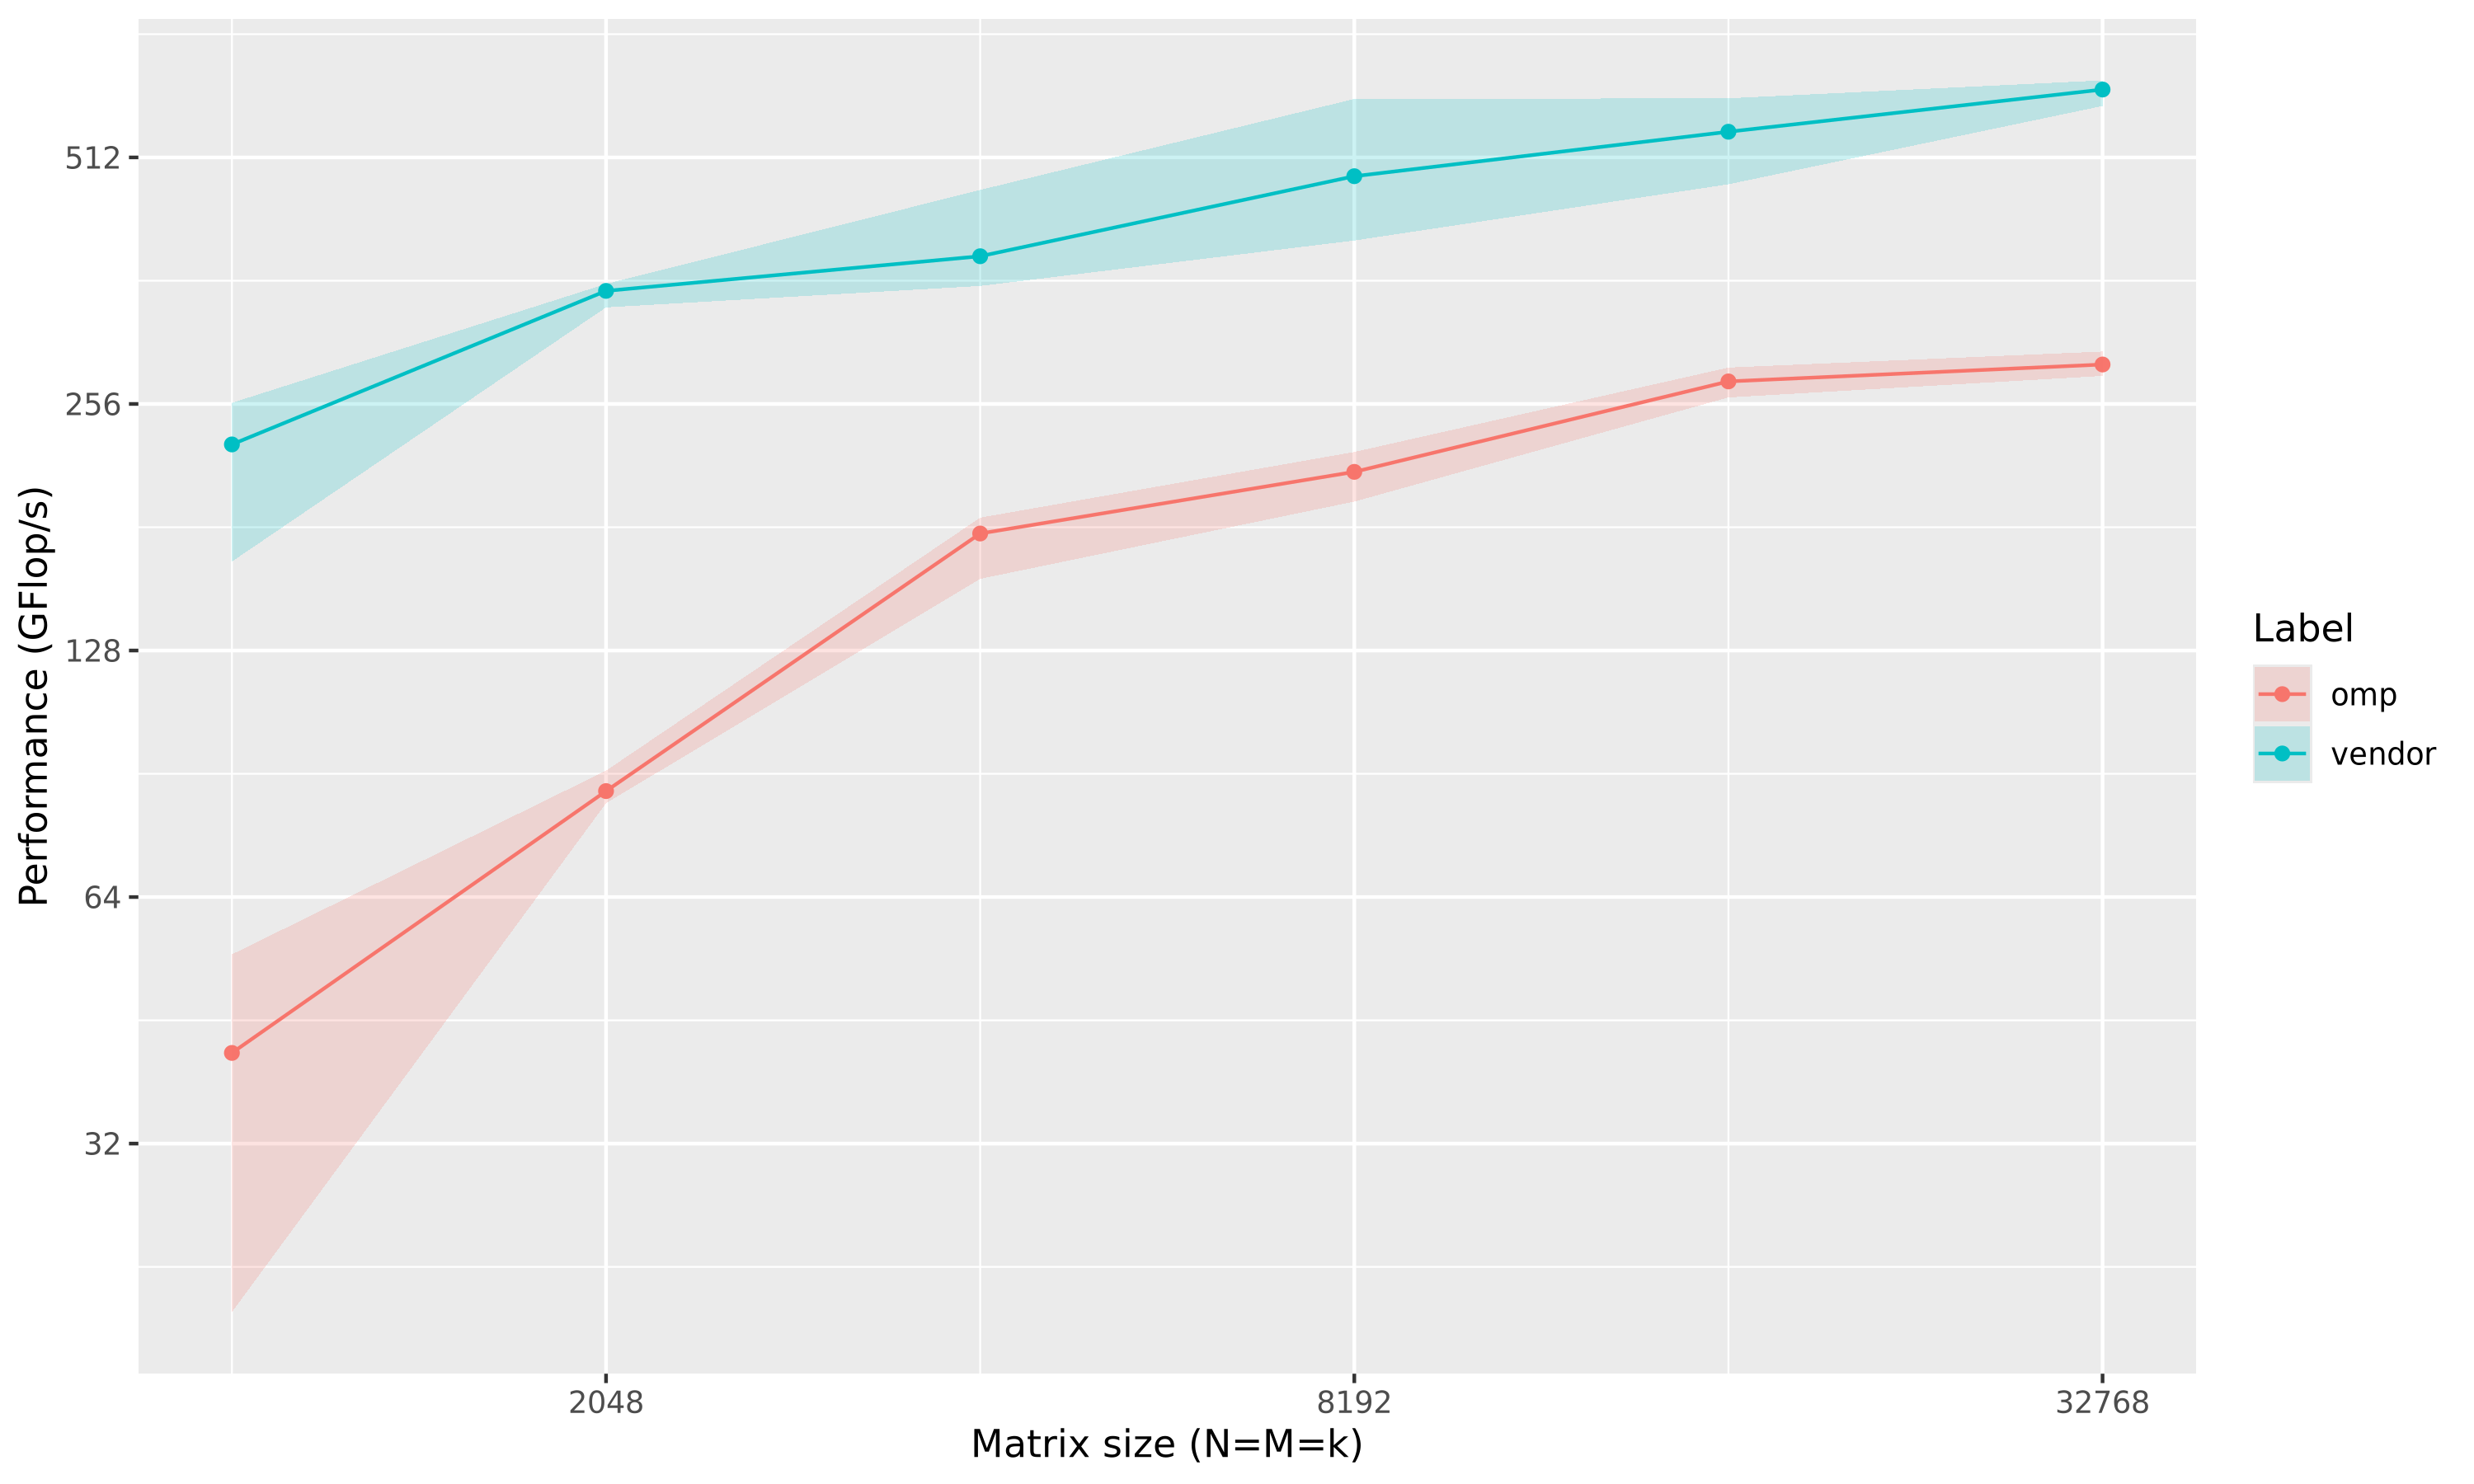
\includegraphics[width=1\textwidth]{assets/gemm_omp.png}
    \caption{Comparaison en mémoire partagée de notre implémentation VS OpenBLAS}
    \label{fig:omp-v-oblas}
\end{figure}

On constate une dynamique similaire à celle que nous avions déjà sur un seul coeur même si nous sommes désormais un peu en dessous de la moitié des performances d'OpenBLAS. Cependant nous ne nous sommes pas attardés sur cette version car la version tuilée a très vite montré de meilleurs résultats.
